\documentclass[hidelinks,12pt]{article}
\usepackage{amsmath}
\usepackage{graphicx}
\usepackage[english]{babel}
\usepackage[utf8]{inputenc}
\usepackage{fancyhdr}
\usepackage{tabularx}
\usepackage{hyperref}
\usepackage{float}
\usepackage{subcaption}
\usepackage{listings}
\usepackage{xcolor}
\usepackage{geometry}
\geometry{a4paper, margin=0.6in}


\definecolor{codegreen}{rgb}{0,0.6,0}
\definecolor{codegray}{rgb}{0.5,0.5,0.5}
\definecolor{codepurple}{rgb}{0.58,0,0.82}
\definecolor{backcolour}{rgb}{0.95,0.95,0.92}

\lstdefinestyle{mystyle}{
    backgroundcolor=\color{backcolour},   
    commentstyle=\color{codegreen},
    keywordstyle=\color{magenta},
    numberstyle=\tiny\color{codegray},
    stringstyle=\color{codepurple},
    basicstyle=\ttfamily\footnotesize,
    breakatwhitespace=false,         
    breaklines=true,                 
    captionpos=b,                    
    keepspaces=true,                 
    numbers=left,                    
    numbersep=5pt,                  
    showspaces=false,                
    showstringspaces=false,
    showtabs=false,                  
    tabsize=2
}

\lstset{style=mystyle}

\hypersetup{
    colorlinks=true,
    linkcolor=cyan,
}

\pagestyle{fancy}
\fancyhf{}
\chead{Assignment-2}
\rfoot{\thepage}
\begin{document}
\begin{titlepage}
  \centering
  
\includegraphics[scale=0.5]{./iitdlogo.png}\\[1.0cm]
  \Large INDIAN INSTITUTE OF TECHNOLOGY DELHI\\[1.0 cm]
  \LARGE COL761\\[0.1cm]
  \Large \underline{Report}\\
  \large \[Assignment-2\]
  % \LARGE \textbf{Model based and Model Free RL}


  \rule{\textwidth}{0.2 mm} \\[0.1cm]
  \begin{abstract}
    The aim of this assignment is to experiment with different frequent subgraph mining algorithms and use this knowlege to design a pipeline for fast querying of subgraphs given an input database of graphs. Additionaly, we also analyze the elbow plot for K-Means algorithm and attempt to explain the number of clusters through it.
    % \\[0.1cm]
  \end{abstract}
  \rule{\textwidth}{0.2 mm} \\[0.1cm]
  \begin{flushright}

    \begin{tabular}{c|c}
      \small {Harsh Agrawal}    & \small {2019CS10431} \\
      \small {Pranjal Aggarwal} & \small {2019CS50443} \\
    \end{tabular}
  \end{flushright}
\end{titlepage}
\newpage
\section{Frequent Subgraph Mining}
\begin{figure}[H]
  \centering
  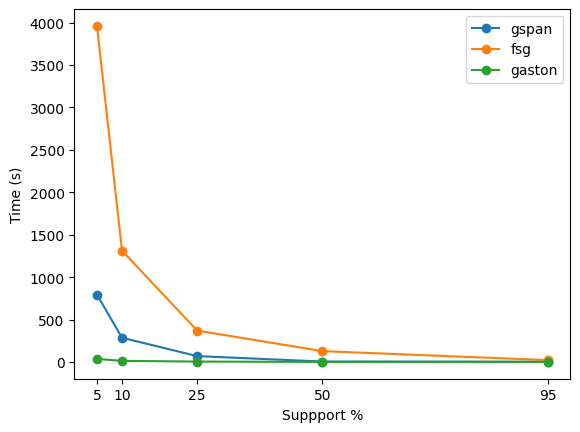
\includegraphics[width=\textwidth]{1.png}
  \caption{Runtimes of various algorithms at changing support level.}
\end{figure}

\begin{itemize}
  \item \textbf{FSG:} It can be clearly observed that the running time of FSG is the highest. This is because it, needs to scan the database for every candidate set and check if they meet the requisite support. Additionally, the canonical labelling can often be very expensive in case of symmetric graphs (which is usually the case with chemical compounds).
  \item \textbf{Gspan:} Gspan requires considerably lower time than FSG, because of its depth first approach and various optimizations that can be applied therein. Being a depth-first algorithm, the space required is much lesser and the cost of I/O operations is considerably lower. Moreover, at increasing depths the number of candidate graphs in the database rapidly shrinks which makes it easier to execute the support test. Also, computing DFS code is relatively cheap than canonical labelling which has no guarantees on the runtime. Note that during join of two k-size subgraphs, FSG considers all possible candidates, whereas Gspan grows the subgraph in a predefined direction, pruning away graphs if they are already checked or are infrequent.
  \item \textbf{Gaston:} It can be observed that the runtime of Gaston is lowest irrespective of the support. This follows from a novel observation that most of the frequent subgraphs are simple and rarely complex in structure. That is to say, simple paths and trees are more common in real-life datasets than complex cylic graphs. Using a novel strategy where graphs are extended in the order path $\rightarrow $ tree $\rightarrow $ graph, it was able to achieve exceptionally low runtimes on the chemical compound dataset.
\end{itemize}
\section{Index structure}

We highlight the approach we used to solve the problem.
\begin{itemize}
  \item Mined frequent subgraphs at a support of \(10\%\). We employed \verb|gaston| \footnote{ Gaston does not output the transaction ids for each subgraph. We patched the source code to also output the transaction ids.}for the task as it was relatively fast.
  \item We built an index structure in the form of a matrix \(M\) where \(M_{ij} = 1\) if \(i^{\text{th}}\) graph contains the \(j^{\text{th}}\) frequent subgraph and \(0\) otherwise.
  \item Additionally, we also built a tree such that a frequent subgraph \(G_p\) is  parent of a frequent subgraph \(G_c\) if \(G_c\) was formed by addition of a single edge in \(G_p\).
  \item During the querying stage, we use the \textbf{Uniform Cost Search} algorithm to expand nodes for subgraph isomorphism tests. The aim is to reduce the number of subgraph isomorphisms using \textbf{VF3} \footnote{The original version of VF3 does not support edge labels, we patched the source code to support edge labels} as much as possible. We start with a priority queue adding all the root node(s) of our tree. The priority queue priortizes node on the value of their support in the database. If for a given subgraph in the priority queue, it is not the subgraph of the query graph then its subtree is not visited and it is simply popped from the queue. Otherwise all of its children are added to the priority queue. At any stage we have the list of all the remaining candidate graphs that have the same features as those currently tested. If at any stage the number of candidates is less than a certain percentage of the number of features left to test, the search is terminated, and subgraph isomorphism is performed on all the remaining candidate graphs.
\end{itemize}
Using the above algorithm we are able to achieve really fast runtimes on the benchmarking datasets that were provided.
\section{Clustering - Elbow Plot}

\begin{figure}[H]
  \centering
  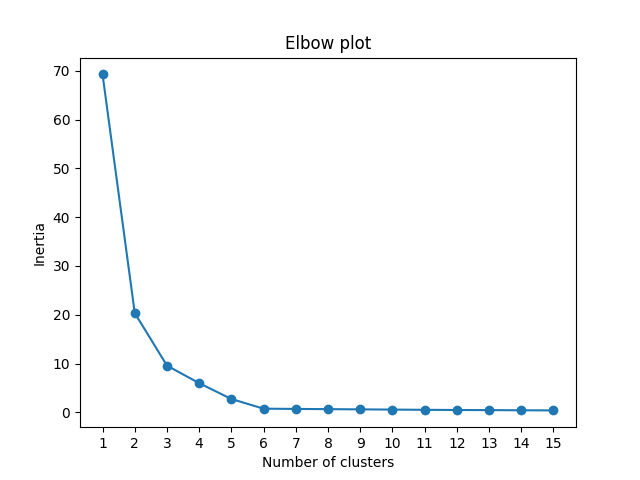
\includegraphics[width=\textwidth]{elbow_4.png}
  \caption{Elbow Plot for \(d = 4\)}
\end{figure}

From the elbow plot it is visible that the inertia rapidly decreases till \(K=6\)
and remains almost constant thereafter. This means the clustering is almost complete when \(K=6\) and any more clusters do not add any value to our clustering and might themselves be very near to each other. Thus \(K=6\) is the optimal number cluster centers value for this dataset.



\end{document}

